
\newcommand{\vdmkw}[1]{\texttt{\textbf{#1}}}
\chapter{Automatic Generation of Code}\label{sec:codegen}

It is possible to generate Java code\index{code generation} for a
large subset of VDM-SL and VDM++ models. In addition to Java, C and
C++ code generators are currently being developed. Both these code
generators are in the early stages of development. For
comparison, code generation of VDM-SL and VDM++ specifications to both
Java and C++ is a feature that is available in
VDMTools~\cite{Java2VDMMan,CGMan,CGManPP}. The majority of this
chapter focuses solely on the Java code generator available in
VDM VSCode Extension.

\section{Use of the Java Code Generator}
\label{sec:javacg_use}

\begin{figure}[htbp]
\begin{center}
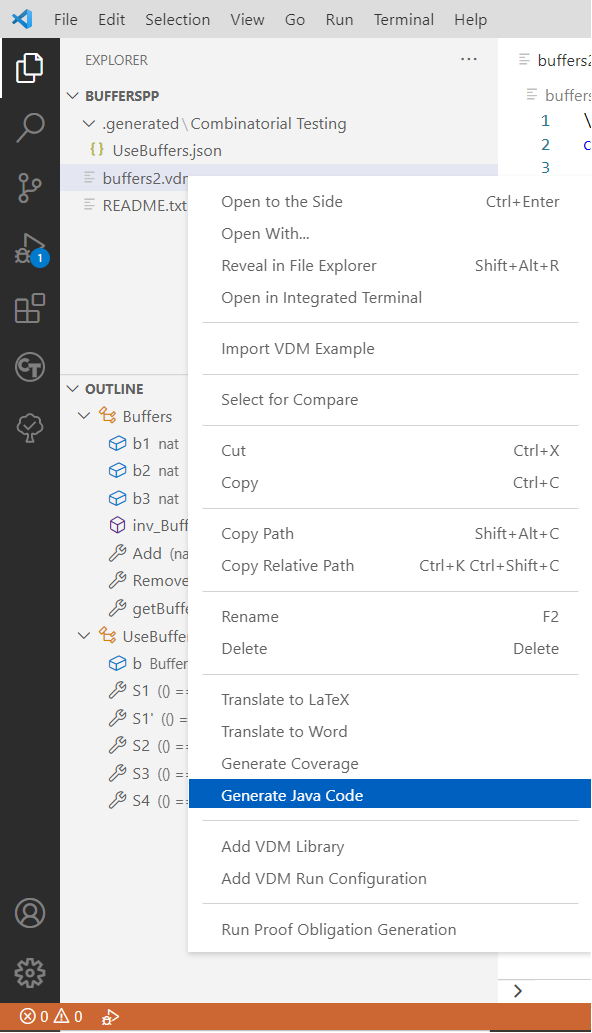
\includegraphics[width=10cm]{snapshots/Launching the java code generator.png}
\caption{Launching the Java code generator.\label{fig:javacg_menu}}
\end{center}
\end{figure}

\begin{figure}[htbp]
\begin{center}
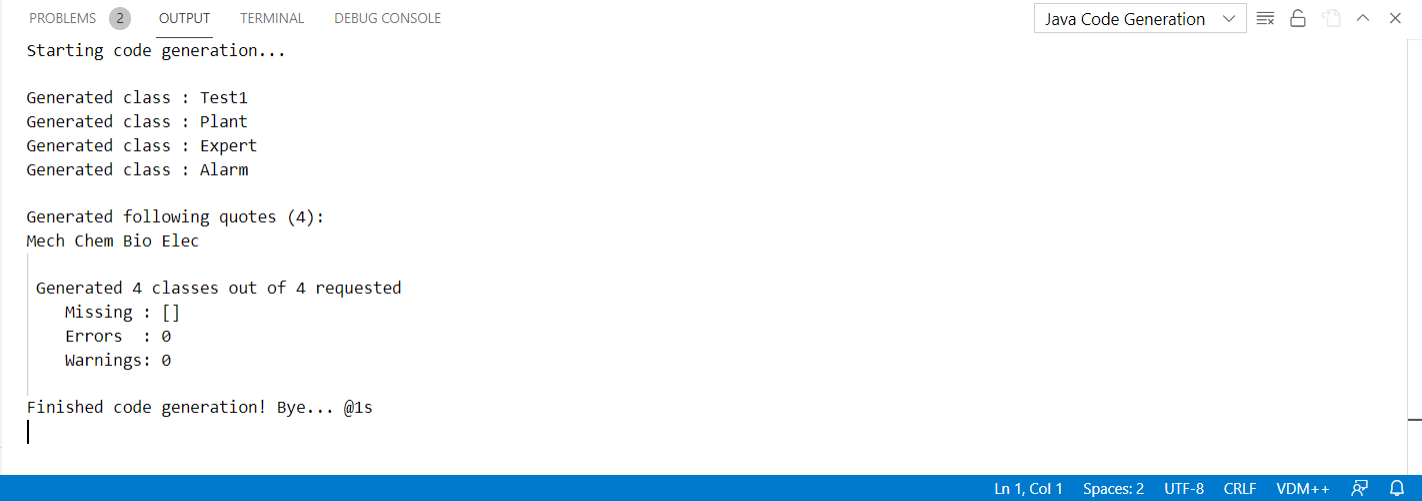
\includegraphics[width=\linewidth]{snapshots/Status of code generating the Alarm PP example.png}
\caption{The status of code generating the \texttt{AlarmPP}
example.\label{fig:javacg_output}}
\end{center}
\end{figure}

The Java code generator can be launched via the context menu as shown
in Figure~\ref{fig:javacg_menu}. Alternatively, this can be done by
highlighting the project in the VDM Explorer and typing one of the
shortcuts associated to this plugin. To launch the Java Code Generation, right click on file and select 'Generate Java Code'.\\


\noindent Upon completion of the code generation process the status is
output to the console as shown in Figure~\ref{fig:javacg_output}. In
particular this figure shows the status of code generating the
\texttt{AlarmPP} model available in the Overture standard examples. As
indicated by the console output, the generated code is available as an
VSCode project in the \texttt{generated/java}
folder.




\section{Limitations of the Java Code Generator}

If the Java code generator encounters a construct that it cannot code
generate it will report it as unsupported to the user and the user can
then try to rewrite that part of the specification using other
(supported) constructs. Reporting of unsupported constructs is done
via the console output and using editor markers.\\

\clearpage
The user will get similar messages and markers for other unsupported
VDM constructs. To summarise, the Java code generator currently does
not support code generation of multiple inheritance and neither does
it support traces, type binds, invariant checks and pre and post
conditions. Furthermore, let expressions appearing on the right-hand
side of an assignment will also be reported as unsupported. The Java
code generator also does not support every pattern. The patterns that
are currently not supported are: object, map union, map, union, set,
sequence, concatenation and match value.

\section{The Code Generation Runtime Library}

The generated code relies on a runtime library used to represent some
of the types available in VDM (tokens, tuples etc.) as well as
collections and support for some of the complex operators such as
sequence modifications. For simplicity every project generated
by the Java code generator contains the runtime library. More
specifically, there is a copy of the runtime library containing only
the binaries (\texttt{lib/codegen-runtime.jar}) as well as a version
of the runtime library that has the source code attached
(\texttt{lib/codegen-runtime-sources.jar}). The runtime library is
imported by every code generated class using the Java import statement
\texttt{\textbf{import} org.overture.codegen.runtime.*;} and in order
to compile the generated Java code the runtime library must be visible
to the Java compiler.

Similar to VDMTools the runtime library also provides implementation
for subset of the functionality available in the standard libraries:
The runtime library provides a full implementation of the
\texttt{MATH} library, support for conversion of values into character
sequences as provided by the \texttt{VDMUtil}, and finally
functionality to write to the console as available in the \texttt{IO}
library.

\newpage
\section{Translation of the VDM types and type constructors}
\label{sec:type-mappings}

Table ~\ref{tbl:type-mappings} describes how the VDM type(s) in the
left column are represented in the generated Java code (the right
column). In this table \texttt{pack} is the user-specified root
package of the generated Java code
and \texttt{E}, \texttt{D} and \texttt{R} represent arbitrary VDM
types. The type mapping in the last row is only used when the
\emph{Generate character sequences as strings} option is selected. Some of the types used to represent the VDM types are native Java types (from package
\texttt{java.lang}), others are part of the Java code generator
runtime library (from package \texttt{org.overture.codegen.runtime}),
and some are generated.

\begin{center}
    \begin{tabular}{| l | l |}
    \hline
    VDM type(s) & Java type \\ \hline
    \vdmkw{bool} & \texttt{java.lang.Boolean} \\ \hline
    \vdmkw{nat}, \vdmkw{nat1}, \vdmkw{int}, \vdmkw{rat}, \vdmkw{real} & \texttt{java.lang.Number} \\ \hline
    \vdmkw{char} & \texttt{java.lang.Character} \\ \hline
    \vdmkw{token} & \texttt{org.overture.codegen.runtime.Token} \\ \hline
    Tuple types (e.g.\ \vdmkw{nat} \texttt{*} \vdmkw{nat}) & \texttt{org.overture.codegen.runtime.Tuple} \\ \hline
    Union types (e.g.\ \vdmkw{nat} \texttt{|} \vdmkw{nat}) & \texttt{java.lang.Object} \\ \hline
    Quote type \texttt{ <T>} & \texttt{pack.quotes.TQuote} \\ \hline
    User-defined types \texttt{T = D} & Represented using the representation of type \texttt{D} \\ \hline
    A class \texttt{C} & \texttt{pack.C} \\ \hline
    Record type \texttt{R} defined in class or module \texttt{M} & Inner class \texttt{pack.M.R}  \\ \hline
    \vdmkw{set of} \texttt{ E} & \texttt{org.overture.codegen.runtime.VDMSet} \\  \hline
    \vdmkw{map} \texttt{ D } \vdmkw{to} \texttt{ R}, \vdmkw{inmap} \texttt{ D } \vdmkw{to} \texttt{ R} & \texttt{org.overture.codegen.runtime.VDMMap} \\  \hline
    \vdmkw{seq of} \texttt{ E}, \vdmkw{seq1 of} \texttt{ E}  & \texttt{org.overture.codegen.runtime.VDMSeq} \\  \hline
    \vdmkw{seq of char}, \vdmkw{seq1 of char} & \texttt{java.lang.String} \\  \hline
    \end{tabular}
  \captionof{table}{The type mappings used by the Java code generator.}
  \label{tbl:type-mappings}
\end{center}
%
%
%
